\documentclass[11pt,dvipdfmx,b5paper,oneside,report,uplatex]{jsbook}


\usepackage{color}
\usepackage{here}
\usepackage{framed}
\usepackage{tcolorbox}
\usepackage{quotchap}
\usepackage{pdfpages}
\usepackage[hidelinks]{hyperref}
\usepackage{pxjahyper}
\usepackage{titlesec}
\usepackage{picture}
\usepackage{tikz}
\usepackage{graphicx}
\usepackage{geometry}
\usepackage{url}


\tcbuselibrary{breakable}
\definecolor{shadecolor}{gray}{0.80}



% section
\titleformat{\section}[block]{}{}{0pt}
{
  \definecolor{teal}{gray}{0.30}
  \begin{picture}(0,0)
    \put(-10,-5){
      \begin{tikzpicture}
        \fill[teal] (0pt,0pt) rectangle (5pt,19pt);
      \end{tikzpicture}
    }
    \put(-10,-5){
      \color{teal}
      \line(1,0){\hsize}
    }
  \end{picture}
  \hspace{0pt}
  \sf \Large \thesection
  \hspace{0pt}
}

% 図表見出し
\renewcommand{\tablename}{\textcolor{gray}{▼} 表}
\renewcommand{\figurename}{\textcolor{gray}{▲} 図}

\begin{document}

\begin{titlepage}
  \newgeometry{left=0cm,right=0cm,top=0cm,bottom=0cm}
  \centering
  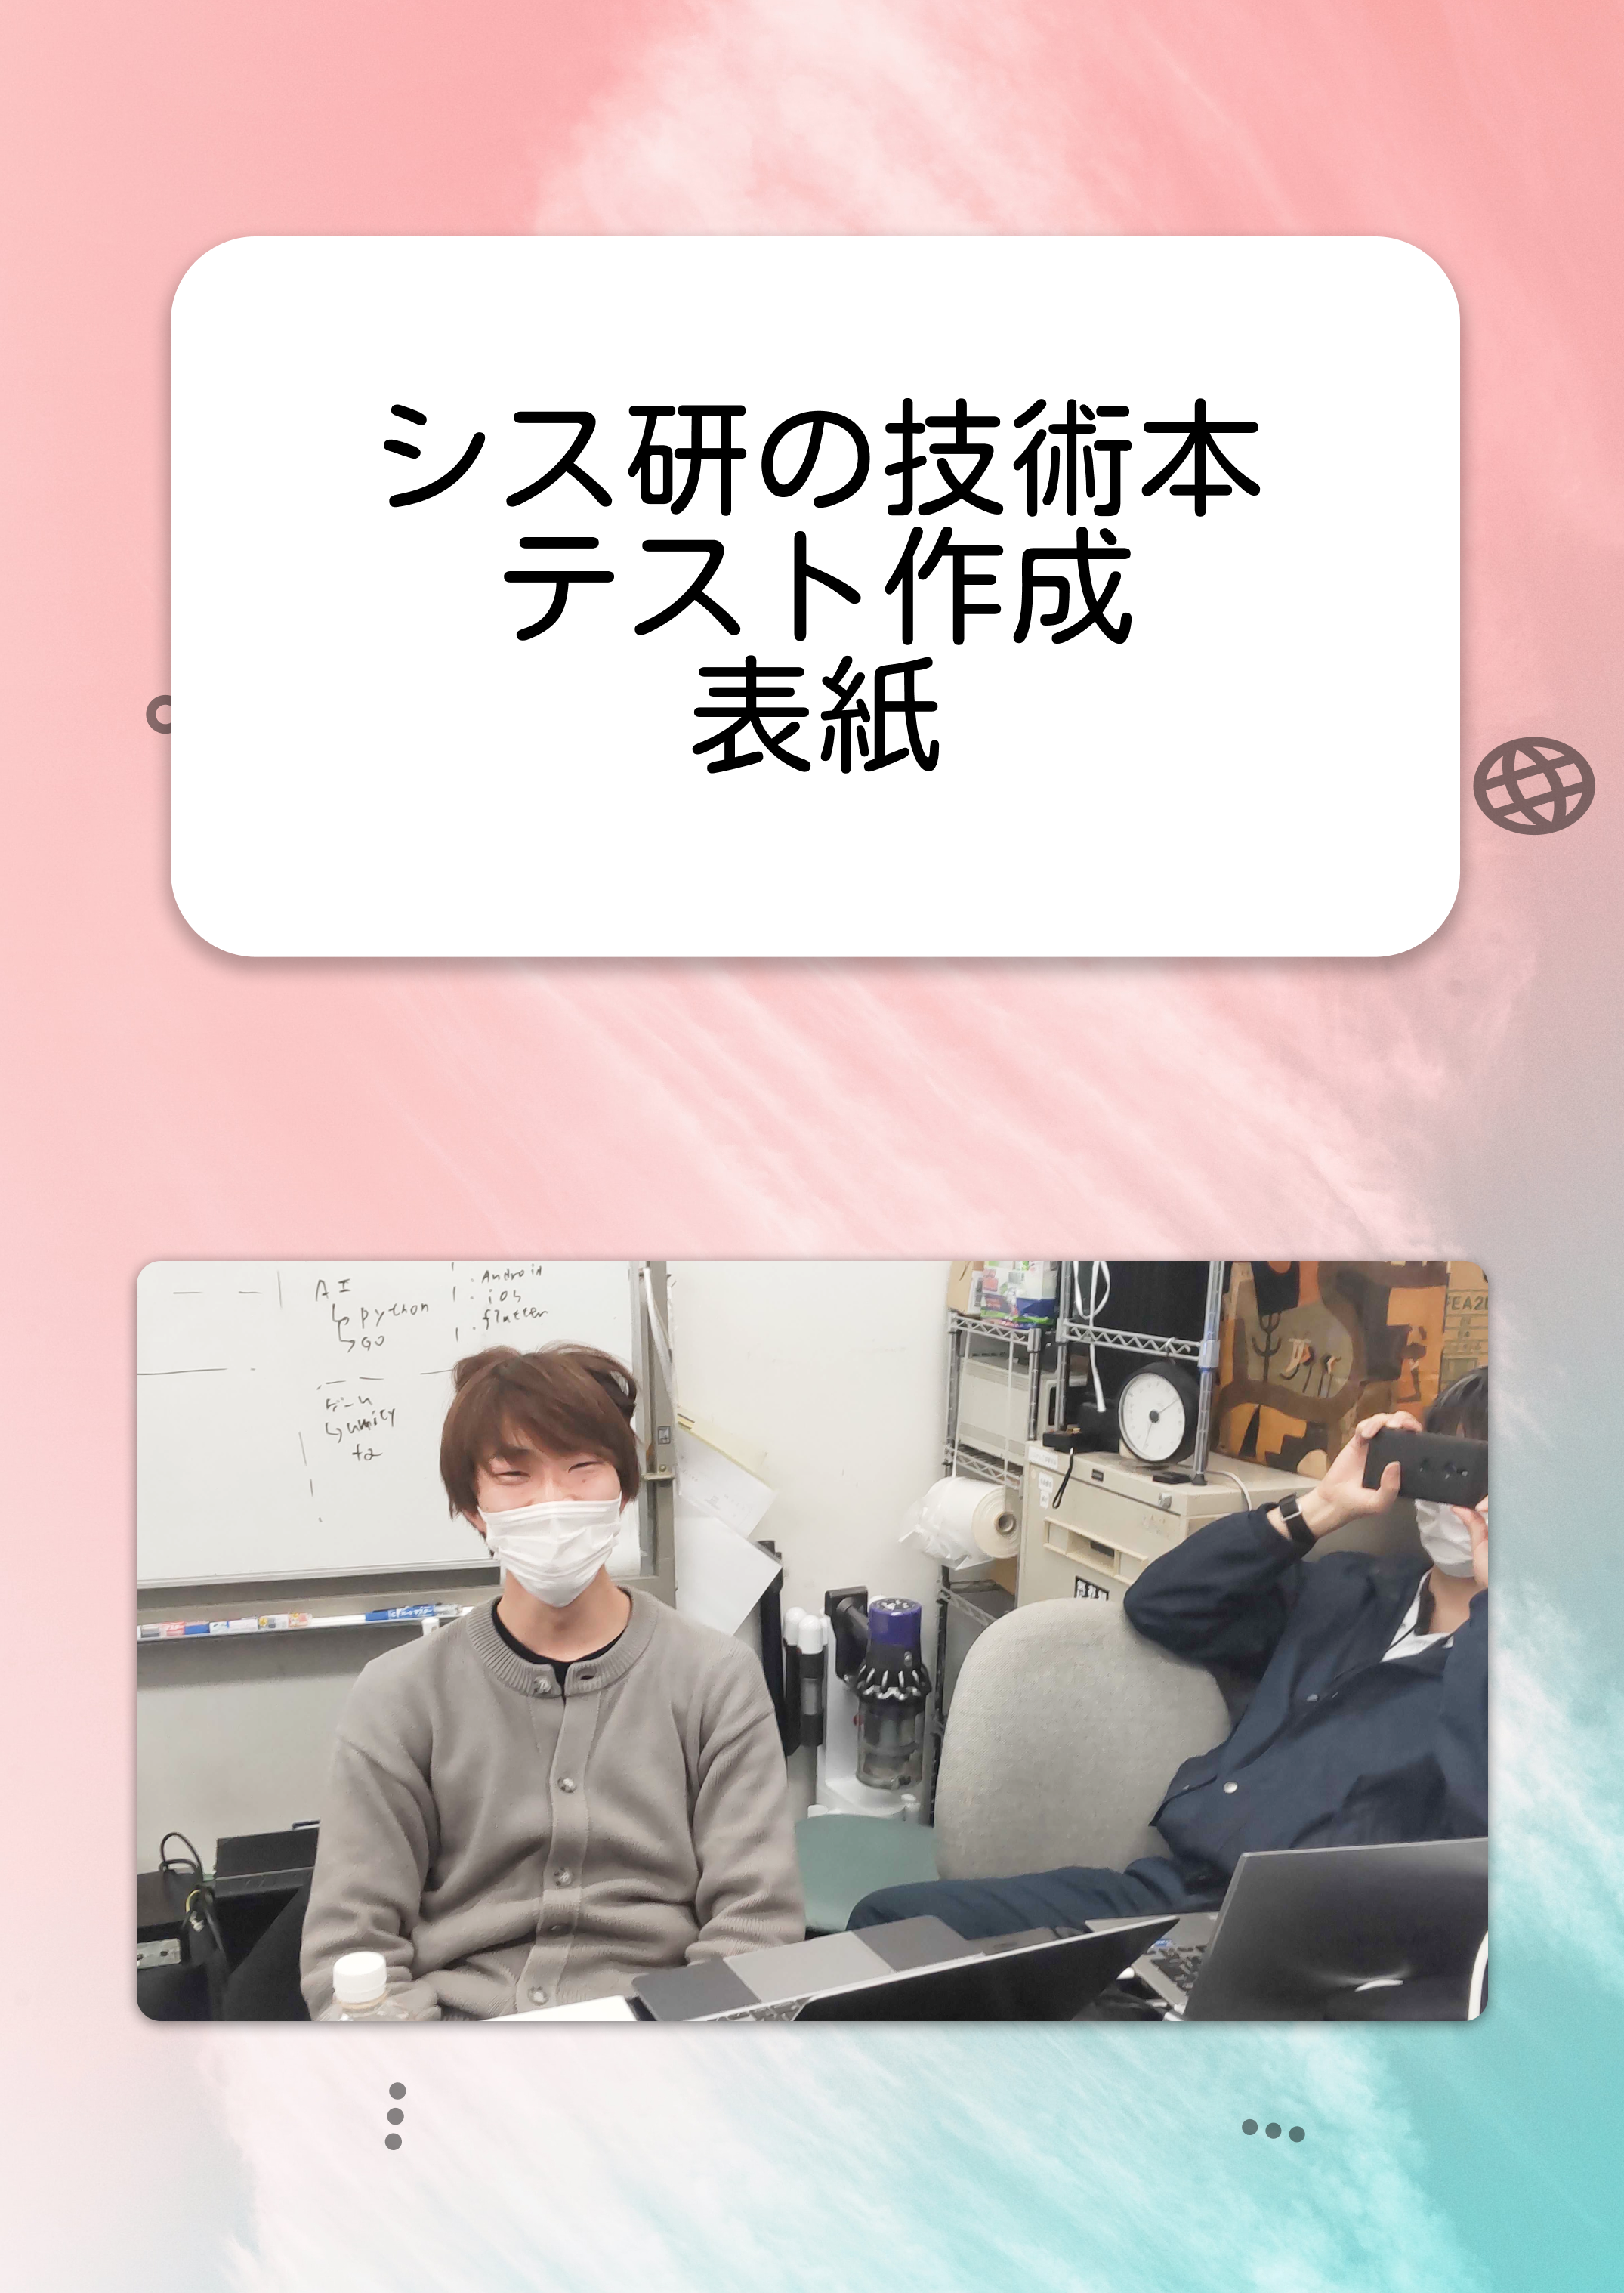
\includegraphics[width=\paperwidth,height=\paperheight]{./image/01-title/titlepage.pdf}
  \restoregeometry % 元の余白に戻す
\end{titlepage}

%目次を自動的に作る。
\tableofcontents

\chapter{シス研というサークルについて}

\section{シス研というサークルについて}
\subsection{はじめに}
初めまして!シス研会長の林です!
はい、ここでみなさんシス研とはなんぞ?となっていると思うのでまずは自分が水先案内人となりましてこの本とシス研について解説していこうと思います。

\subsection{どんな話をするのか}
シス研ってどんなサークル?どんな活動をしているの?この本はどういったもの?といったものを紹介していきます。それでは、さっそく行ってみましょう!!!

\section{シス研とは}
シス研は正式名称を「システム工学研究会」と言い、愛知工業大学公認の情報系サークルです。歴史は長く、2023年で創立47周年を迎え、かのAppleと同い年となります!! \\
シス研ではハッカソン出場をはじめとしたチーム開発、ゲーム作成、インフラの構築、運用などを行っています。

\subsection{どんな活動をしているの?}
シス研の主な活動はチーム開発とインフラ整備です。サークル全体としての開発物などはなく、それぞれがチームを組んでハッカソンに出場したりしています。 \\
インフラ面では、部室に物理サーバを持っており、そこでシス研のホームページや各種サービスを公開しています。\footnote{シス研ホームページ\url{https://set1.ie.aitech.ac.jp}}\footnote{シス研紹介ページ\url{https://welcome.sysken.net}}23年4月現在、大幅な工事を行なっておりごく一部のサービスのみ稼働しています(すみません)
そのほかにもシス研主催のLT会・ハッカソンの開催、Qiitaアドベントカレンダーへの参加もしています。\footnote{Advent Calendar 2022 \url{https://qiita.com/advent-calendar/2022/stech-ait-advent}}

\begin{figure}[bht]
  \centering
  \includegraphics[width=10cm]{./image/02-AboutSysken/room.jpg}
  \caption{部室の様子}
\end{figure}

\subsection{21〜22年度の活動実績}
\begin{itemize}
  \item 2021 愛工大大学祭 工科展 最優秀賞
  \item 2022 技育博 参加
  \item 2022 Geekcamp vol8 優秀賞
  \item 2022 愛工大大学祭 工科展 瑞若賞
  \item 2022 技育展 出展
  \item 2022 愛工大大学祭 模擬店 最優秀賞
  \item 2022 HackU 春・夏 参加
  \item 2022 Geekcampアドバンス 登壇
  \item 長期休暇中のLT会、ハッカソン主催
  \item 各種勉強会の開催
\end{itemize}

\begin{tcolorbox}[title=シス研の設備]
  \begin{itemize}
    \item ブレードサーバ、ネットワーク機器
    \item デスクトップPC
    \item iMac,MacBook
    \item iPhone,iPad
    \item Android端末各種
    \item Raspberry Pi
    \item はんだ等の電子工作セット
    \item その他多数...
  \end{itemize} 
\end{tcolorbox}

\begin{figure}[H]
  \begin{tabular}{cc}
    \begin{minipage}[b]{0.40\columnwidth}
      \centering
      \includegraphics[width=\columnwidth]{./image/02-AboutSysken/server.jpg}
      \caption{ブレードサーバ}
    \end{minipage} &
    \hspace{0.04\columnwidth}
    \begin{minipage}[b]{0.40\columnwidth}
      \centering
      \includegraphics[width=\columnwidth]{./image/02-AboutSysken/network.jpg}
      \caption{ネットワーク機器}
    \end{minipage} \\
    \begin{minipage}[b]{0.40\columnwidth}
      \centering
      \includegraphics[width=\columnwidth]{./image/02-AboutSysken/iPad.jpg}
      \caption{タブレット端末}
    \end{minipage} &
    \hspace{0.04\columnwidth}
    \begin{minipage}[b]{0.40\columnwidth}
      \centering
      \includegraphics[width=\columnwidth]{./image/02-AboutSysken/RaspberryPi.jpg}
      \caption{Raspberry Pi}
    \end{minipage}
  \end{tabular}
\end{figure}

\section{この本について}
この本はシス研のメンバーが経験したこと、取り組んだことのアウトプットを目的としたものです。この本を通じて皆さんにはシス研のメンバーは具体的にどのような活動をしているのか知ってもらいたいと思います。 \\
また、シス研として本を出すのは今回が初めてなのでどうか温かい目で見ていただけると幸いです。

\section{まとめ}
ここまでお話をして来ましたが簡単にでもシス研について知ってもらうことはできたでしょうか?うまく伝えることができていたらとても嬉しいです。 \\
次のページからはメンバーの記事本編になります!シス研初めての本をよろしくお願いします!!
\chapter{DiscordBotを作ってみよう!}

\section{DiscordBotを作ってみよう}
\subsection{はじめに}
初めに今回何故DiscordのBotを作ろうと思ったかの経緯をお話しします。
私はDiscordで人とチャットをしている時に同じ会話が頻繁に続き、これBotで返事を返すようにしたら返事を返す手間が省けるし面白いのでは?と思ったのがBotを作ろうと思ったきっかけです。
発想がひどいって!?まあでも自分の発想したものを形にすることが面白いことだと思うので今回はそこには目を瞑りましょう…
もちろん自分が送ったメッセージに対してBotに返答させることもできるので、自分だけのオリジナルDiscordBotを作ってみましょう!

\subsection{何を作るのか}
Discordのサーバで特定のメッセージが来たら、特定のメッセージを返すDiscordのBotを作ります。

\section{実行環境・使用技術・ソースコードの管理}
\subsection*{実行環境}
調べる必要あり
\subsection*{使用技術等}
\begin{itemize}
  \item Python(discord.py)を使用
  \item Flaskを用いてWebサーバを構築
\end{itemize}
\subsection*{ソースコードの管理}
\begin{itemize}
  \item Git・GitHubを使用
  \item .envファイルをGitHubにアップロードしないようにする
\end{itemize}

\section{ローカル環境でBotが動作するようにする}
まずはローカル環境でBotが動作するようにしてみます。

\subsection{Botの作成・管理をする}
初めに機能などはまだついていないBotをDiscordのポータルサイトから作成します。
DiscordのBotの作り方(メモ)という記事の「1.Discord上のBotの作成」を見ながらBotを作成してみて下さい。
\footnote{引用した記事についての注釈を書く}。
同記事内の「2.Glitchでサーバーを作成」の部分は、今回Glitchは使用しないため行う必要はありません。

\subsection{Pythonの確認}
先ほど作成したBotをDiscordのサーバーに招待することができたらPythonが使えるかどうかの確認をしましょう。
Pythonを用いて先ほど作成したBotに機能をつけていきます。\\
今回はPythonの3.x系で実装します。\\
まずは、ローカル環境のPythonのバージョンを調べます。\\
\begin{shaded}
\begin{verbatim}
python --version
\end{verbatim}
\end{shaded}
この状態で2.x系のバージョンが出てくる場合は、下記のコマンドで3.x系のバージョンが出てくるか調べます。
\begin{shaded}
\begin{verbatim}
python3 --version
\end{verbatim}
\end{shaded}
今回はPython3.x系を利用するので3.xのバージョンが出たほうで実装を進めてください。\\
また、discord.pyについては3.8以降で動作します。3.8より前のバージョンが表示されている場合は、最新版のPythonをインストールしてください。

\section{本番環境へデプロイする}

\begin{tcolorbox}[breakable]
\begin{verbatim}
1  /* ここにはソースコードを書く */
2  #include<stdio.h>
3
4  int main(void)
5  {
6    printf("Hello, World!\n");
7    return 0;
8  }
9  /* breakableを付けるとこんな感じで改行にも対応できる */
\end{verbatim}
\end{tcolorbox}

\begin{shaded}
\begin{verbatim}
## ここにはコマンドを書く
$ echo "Hello, World!"
\end{verbatim}
\end{shaded}

図表はキャプションを付けたときに、先頭に「▲」や「▼」を付けるようにした。

\begin{table}[H]
  \centering
  \caption{表のサンプル}
  \begin{tabular}{|c|l|l|l|} \hline
    日本 & hoge & fuga & piyo \\ \hline
    アメリカ & foo & bar & baz \\ \hline
  \end{tabular}
  \label{table-sample0301}
\end{table}

\begin{figure}[H]
  \centering
  \includegraphics[width=4cm]{./image/03-Tech/chap1/sample.png}
  \caption{画像のサンプル}
  \label{figure-sample0301}
\end{figure}

\begin{tcolorbox}[title=これはコラム]
  コラムも随時挟めるようにした。

  tcolorboxはtitleを指定するといい感じにタイトル付きの枠で囲ってくれる。
\end{tcolorbox}
\chapter{リポジトリ作成後に設定しておきたいこと}
\section{はじめに}
こんにちは。hihumikanです。

本チャプターでは「リポジトリ作成後に設定しておきたいこと」をご紹介します。
私自身が次回プロジェクト開始する際に、こういった設定をするだろうというものをまとめました。

ただし、これら全ての内容をプロジェクトに適用出来るものではないため、ご利用の環境や用途に合わせて利用していただければと思います。

\subsection{対象読者}

対象読者は、Git/GitHubを利用した開発を行う初学者の方を想定しています。

\section{ファイルの設定}

リポジトリ作成後に設定しておきたい「ファイルの設定」についてご紹介します。

\subsection{.gitignore}

.gitignoreは、Gitによる管理から除外したいファイルやディレクトリを指定するための設定ファイルです。

例えば、MacOSの場合、ディレクトリ毎に.DS\_Storeというファイルが自動的に生成されます。
このファイルは、ディレクトリのmeta情報を記録しますが、通常の開発において共有する必要がないため、Gitの管理対象外としておくことが望ましいです。

また、.envなどの環境変数を利用してプログラムを動かす場合、.envファイルには、パスワードや秘密鍵などの情報が含まれていることが多いため、これもGitの管理対象外としておくことが望ましいです。

リスト1.1のようなテキストファイルをGitの管理下に置くだけで、Gitから管理対象外として扱うことができます。

\begin{tcolorbox}[title=リスト1.1 .gitignore]
  \begin{verbatim}
1 .DS_Store
2 .env
\end{verbatim}
\end{tcolorbox}

リポジトリを共有する場合、.gitignoreファイルを共有することで、開発メンバー全員が同じ設定を利用できるため、必要なファイルだけがGitの管理下に置かれるようになります。

\subsection{.gitattributes}

.gitattributesは、特定のファイルに対してGitの挙動を変更するための設定ファイルです。
主に、改行コードやファイルの文字コードを指定することが多いです。改行コードの指定は、Windows(CRLF)とLinux(LF)の違いを吸収するために行います。


\subsection{Makefile}


\section{インフラ回り}

\subsection{GitHub Actions}
\subsection{renovate}
\subsection{webhooks}


\section{おわりに}
本チャプターでは「リポジトリ作成後に設定しておきたいこと」をご紹介しました。

\section{参考文献}
\begin{itemize}
  \item \href{https://git-scm.com/docs/gitignore}{gitignore}
  \item \href{https://git-scm.com/docs/gitattributes}{gitattributes}
\end{itemize}


\chapter{DiscordBotを作ってみよう}
\section{はじめに}
はじめまして、sudaです。私はDiscordで人とチャットをしている時に同じ会話が頻繁に続き、これBotで返事をするようにしたら返事をする手間が省けるし面白いのでは?と思いBotを作ることにしました。
発想がひどいって!?まあでも自分の発想したものを形にすることが面白いことだと思うので今回はそこには目を瞑りましょう…
もちろん自分が送ったメッセージに対してBotに返答させることもできるので、自分だけのオリジナルDiscordBotを作ってみましょう!

\section{何を作るのか}
Discordのサーバで特定のメッセージが来たら、特定のメッセージを返すDiscordのBotを作ります。
サンプルプログラムを参照したい方は以下のURLからご覧下さい。
\footnote{今回作るDiscordBotのサンプルプログラム\url{https://github.com/sudamichiyo/Discord_Bot_sampleprogram}}
例えば自分が「仕事終わった」と言うとBotが「お疲れ様」と返してくれます。
\section{実行環境・使用技術}
\begin{itemize}
  \item Python 3.10.8
\end{itemize}


\section{ローカル環境でBotが動作するようにする}
まずはローカル環境でBotが動作するようにしてみます。

\subsection{Botの作成・管理をする}
初めに、機能などはまだついていないBotをDiscordのポータルサイトから作成します。
DiscordのBotの作り方(メモ)という記事の「1.Discord上のBotの作成」を見ながらBotを作成してみて下さい。
\footnote{DiscordのBotの作り方(メモ)\url{https://note.com/exteoi/n/nf1c37cb26c41 (参照2023.3.29)}}

\subsection{ファイルの作成}
Botを実行するPythonファイルを作ります。
\begin{shaded}
  \begin{verbatim}
$ mkdir message_discord_bot
$ cd message_discord_bot
$ touch main.py
\end{verbatim}
\end{shaded}

\subsection{discord.pyの準備}
ここからはライブラリ(discord.py) のドキュメントを見ながら環境構築をしていきます。
\footnote{discord.pyドキュメント\url{https://discordpy.readthedocs.io/ja/latest/intro.html\#basic-concepts (参照2023.3.29)}}
PythonでDiscordのAPIを操作するために必要なライブラリをインストールします。先ほど作成したディレクトリにアクセスして、以下のコマンドで discord.py をインストールします。
\begin{shaded}
  \begin{verbatim}
$ python3 -m pip install -U discord.py
\end{verbatim}
\end{shaded}
次に、先ほど作成したmain.pyを以下のソースコードに書き換えます。
\begin{tcolorbox}[breakable]
  \begin{verbatim}
1 import discord
2 
3 class MyClient(discord.Client):
4     async def on_ready(self):
5         print(f'Logged on as {self.user}!')
6 
7     async def on_message(self, message):
8         print(f'Message from {message.author}
9                                         : {message.content}')
10
11 intents = discord.Intents.default()
12 intents.message_content = True
13
14 client = MyClient(intents=intents)
15 client.run('my token goes here')
\end{verbatim}
\end{tcolorbox}
ここで、以下のボットに関する2つの設定をDiscordのポータルサイトから設定してください。
\begin{itemize}
  \item ポータルサイトの「Bot」からトークンを取得する
  \item ポータルサイトの「Bot」の「MESSAGE CONTENT INTENT」を有効にする
\end{itemize}
'my token goes here'は取得したBotのアクセストークンを書きます。
以上の設定が終わったところで python3 main.py を実行すると、Botのサーバが立ち上がります。Bot のいるサーバの任意のチャンネルでメッセージを投稿すると
、コマンドライン上に「書いた人」と「メッセージ」がそのまま出力されます。

\subsection{環境変数の設定}
ソースコードに直接トークンを書いてしまうと、Githubでソースコードをホスティングするときにトークンキーが他の人にバレてしまいます。
これを防ぐために.envファイルを作成して、その中にDiscordのアクセストークンを書きます(下記参照)。
\begin{tcolorbox}[breakable]
  \begin{verbatim}
1 DISCORD_TOKEN='My token goes here'
\end{verbatim}
\end{tcolorbox}
Pythonの中で.envファイルに書かれている変数を取得するために dotenv というライブラリを使用します。以下のようにインストールします。
\begin{shaded}
  \begin{verbatim}
$ pip3 install python-dotenv
\end{verbatim}
\end{shaded}
インストール後にmain.pyに下記のコードを付け加えて下さい。\\
main.pyのimport discordとclass MyClientの間に以下のコードを追加します。
\begin{tcolorbox}[breakable]
  \begin{verbatim}
1 import os
2 from dotenv import load_dotenv
3 load_dotenv()
\end{verbatim}
\end{tcolorbox}
そして、最後の行を以下のように書き換えて下さい。
\begin{tcolorbox}[breakable]
  \begin{verbatim}
1 client.run(os.environ['DISCORD_TOKEN'])
\end{verbatim}
\end{tcolorbox}
書き換えたあとに python3 main.py を実行すると,先ほどと同じようにメッセージの受け取りをしてくれるサーバーサイドアプリケーションが立ち上がります。

\subsection{Botが特定のワードに反応して、特定のメッセージを返答する機能をつける}
プログラムを起動して正常にサーバーサイドアプリケーションがメッセージを受け取れるようになったら、Botが特定のワードに反応して、特定のメッセージを返答する機能をつけていきます。
Botに機能をつけるには上記のソースコードの8行目と10行目の間に以下のコードを付け足していきます。\\
\begin{tcolorbox}[breakable]
  \begin{verbatim}
1 # メッセージを書いた人がBotなら処理終了
2 if message.author.bot:
3     return
4 channel = message.channel 
5 if message.content == '仕事終わった':
6     await channel.send('お疲れ様')
\end{verbatim}
\end{tcolorbox}
付け足したコードの解説をしていきます。\\
2,3行目でメッセージを書いた人がBotなら処理を終了させています。\\
4行目でメッセージが投稿されたチャンネルを取得しています。\\
5行目のmessage.contentはメッセージの内容で、今回の場合「仕事終わった」というメッセージをチャンネルに投稿すると、メッセージが投稿されたチャンネルにBotが「お疲れ様」と返答します。



\begin{figure}[H]
  \centering
  \includegraphics[width=12cm]{./image/03-Tech/chap1/bot.png}
  \caption{動作例}
\end{figure}
\section{まとめ}
今回はDiscordのBotの作り方を説明しました。上記の「仕事終わった」や「お疲れ様」に当たる部分を変えたりして自分好みに改良してみて下さい。

\lstdefinelanguage{JavaScript}{
  keywords={const, let, var, export, default, function, return, if, else, while, for, switch, case, break, throw, catch, typeof, instanceof, import},
  keywordstyle=\color{blue}\bfseries,
  ndkeywords={class, export, boolean, throw, implements, import, this},
  ndkeywordstyle=\color{darkgray}\bfseries,
  identifierstyle=\color{black},
  sensitive=false,
  comment=[l]{//},
  morecomment=[s]{/*}{*/},
  commentstyle=\color{purple}\ttfamily,
  stringstyle=\color{red}\ttfamily,
  morestring=[b]',
  morestring=[b]",
}

\lstdefinelanguage{TypeScript}{
  keywords={const, let, var, export, default, function, return, if, else, while, for, switch, case, break, throw, catch, typeof, instanceof, import, as, type, keyof, typeof, this},
  keywordstyle=\color{blue}\bfseries,
  ndkeywords={class, interface, enum, extends, implements, readonly, abstract, static, public, private, protected, any, boolean, number, string, object, unknown, null, void, never},
  ndkeywordstyle=\color{darkgray}\bfseries,
  identifierstyle=\color{black},
  sensitive=false,
  comment=[l]{//},
  morecomment=[s]{/*}{*/},
  commentstyle=\color{purple}\ttfamily,
  stringstyle=\color{red}\ttfamily,
  morestring=[b]',
  morestring=[b]",
}

\lstdefinestyle{customstyle}{
  language=TypeScript,
  basicstyle=\ttfamily,
  breaklines=true,
  breakatwhitespace=false,
  columns=fullflexible,
  keepspaces=true,
}



\chapter{Next.js 13 触ってみた}
\section{はじめに}
10 月後半に行われた Next.js Conf 2022 で発表された Next.js 13 を実際に触って
みたのでその内容を書きます。当初は全体を網羅して書く予定だったのですが量が多
かったの少し絞ってます。対象読者としてある程度 React や Next.js を触っている
人を対象としています


\section{プロジェクト作成からサーバ起動}

TypeScriptとESLintを入れるか聞かれるので入れる
\begin{tcblisting}{listing only, breakable}
  npx create-next-app@latest --ts
\end{tcblisting}



pagesディレクトリを削除
\begin{tcblisting}{listing only, breakable}
  rm -rf pages
\end{tcblisting}

appディレクトリを作る
\begin{tcblisting}{listing only, breakable}
  mkdir app
\end{tcblisting}


appディレクトリは実験段階の機能なので、next.config.jsを変更する

\begin{tcblisting}{listing only, breakable}
  const nextConfig = {
  reactStrictMode: true,
  swcMinify: true,
  experimental: {
  appDir: true,
  },
  };
\end{tcblisting}

app/page.tsxを作り、以下のようにする



\begin{tcblisting}{listing only, breakable}
  export default function Page() {
      return <h1>Hello, Next.js!</h1>;
    }
\end{tcblisting}




ローカルサーバ起動


\begin{tcblisting}{listing only, breakable}
  npm run dev
\end{tcblisting}



ブラウザで http://localhost:3000/ にアクセスすると、Hello, Next.js! が表示される

\begin{figure}[H]
  \centering
  \includegraphics[width=12cm]{./image/03-Tech/chap4/01.png}
\end{figure}




\section{LayoutとHead
 }

サーバを起動すると自動的にappディレクトリにlayout.tsx,head.tsxというファイルが作られていました。

next/headを使って各ページファイルにheadを定義していたのがhead.tsxに書けるようになったみたいですね

\begin{tcblisting}{listing options={style=customstyle},listing only, breakable}
  export default function Head() {
      return (
      <>
      <title></title>
      <meta content="width=device-width, initial-scale=1" name="viewport" />
      <link rel="icon" href="/favicon.ico" />
      </>
      )
    }
\end{tcblisting}



ページの共通レイアウトを定義するファイル




\begin{tcblisting}{listing options={style=customstyle},listing only, breakable}
  export default function RootLayout({
      children,
    }: {
  children: React.ReactNode
  }) {
      return (
      <html>
        <head />
        <body>{children}</body>
      </html>
      )
    }

\end{tcblisting}


今までは\_app.tsxなどに下記のようにレイアウトを定義していました
\begin{tcblisting}{listing options={style=customstyle},listing only, breakable}
  <Layout>
  <Component {...pageProps} />
  </Layout>
\end{tcblisting}




この方法だとページごとにレイアウトを変えることができません。なのでページごとにレイアウトを変えたい場合はgetLayoutを用いる必要がありました。Next.js 13ではレイアウトを変えたいページがあるディレクトリにlayout.tsxを置くことでページごとにレイアウトを変えることができるようになりました。


ここではダッシュボードページのレイアウトの場合を考えます。
appディレクトリの中でdashbordディレクトリを作成して以下のようにlayout.tsxを配置するだけです。


\begin{tcblisting}{listing options={style=customstyle},listing only, breakable}
  export default function DashboardLayout({
      children,
    }: {
  children: React.ReactNode;
  }) {
      return <section>{children}</section>;
    }
\end{tcblisting}




少し疑問に思ったのがdashboardディレクトリのpage.tsxではRootLayoutは呼ばれずDashboardLayoutのみが呼ばれるのかと思っていました。しかしそんなことはなく入れ子構造で呼び出されるようです。

公式の画像がわかりやすいので貼っておきます。
次の機能に行く前にdashboardディレクトリにpage.tsxも作っておきます
\begin{figure}[H]
  \centering
  \includegraphics[width=12cm]{./image/03-Tech/chap4/02.png}
\end{figure}


\begin{tcblisting}{listing options={style=customstyle},listing only, breakable}
  export default function DashBoardPage() {
      return <h1>DashBoard Page</h1>;
    }

\end{tcblisting}


違いがわかりやすいように他のファイルも変更します\\
app/layout.tsx
\begin{tcblisting}{listing options={style=customstyle},listing only, breakable}
  export default function RootLayout({
      children,
    }: {
  children: React.ReactNode;
  }) {
  return (
  <html>
  <head />
  <body
  style={{
      backgroundColor: '#C0C0C0',
      padding: '50px',
    }}
  >
    {children}
  </body>
  </html>
  );
  }

\end{tcblisting}



app/dashboard/layout.tsx
\begin{tcblisting}{listing options={style=customstyle},listing only, breakable}
  export default function DashboardLayout({
      children,
    }: {
  children: React.ReactNode;
  }) {
  return (
  <section
  style={{
      backgroundColor: 'white',
    }}
  >
    {children}
  </section>
  );
  }
\end{tcblisting}



ページの見た目が画像のようになってればOK


\begin{figure}[H]
  \centering
  \includegraphics[width=12cm]{./image/03-Tech/chap4/03.png}
\end{figure}










\section{React Server Components}
React Server Components(RSC)はReact18で追加された機能でクライアントと
サーバ側が協調してアプリケーションをレンダリングできる機能です。
これによりコンポーネントごとに最適なレンダリング方法を選択できるようになります。
例えばデータの取得はサーバ側で行い、ユーザの操作によって変わる部分はクライアント側で
レンダリングするといったことができます。これも公式ドキュメントの図がわかりやすいので貼っておきます。


\begin{figure}[H]
  \centering
  \includegraphics[width=12cm]{./image/03-Tech/chap4/04.png}
\end{figure}



またSSRとの違いとしてクライアント側のJavaScriptの量を減らせる点です。
SSRの場合ハイドレーション(サーバ側で生成したDOMとクライアントで生成したDOMを合成する)というステップがありページを早く表示できてもクライアント側でも同じ処理が走るためJavaScriptの量は同じでした。RSCはサーバ側でレンダリングした後残りをクライアント側でレンダリングします。これによってクライアント側に送信されるJavaScriptの量を減らすことができます。


\section{サーバーコンポーネントでデータを取得}


appディレクトリ内のコンポーネントはデフォルトだとサーバコンポーネントになっています。
以下のコードはサーバサイドでqiitaの記事リスト取得して表示するものです。
dashboard/page.tsxを書き換えます。



\begin{tcblisting}{listing options={style=customstyle},listing only, breakable}
  type Article = {
  id: number;
  title: string;
  };

  async function getArticle(): Promise<Article[]> {
  const res = await fetch('https://qiita.com/api/v2/items?page=1&per_page=24');

  if (!res.ok) {
      throw new Error('Failed to fetch data');
    }

  return res.json();
  }

  export default async function DashBoardPage() {
  const articles = await getArticle();

  return (
  <div>
  <h1>Dashboard</h1>
  <div
  style={{
      display: 'flex',
      flexDirection: 'column',
      flexWrap: 'wrap',
      height: '50vh',
    }}
  >
  {articles?.map((article) => (
  <div
  key={article.id}
  style={{
      display: 'flex',
      gap: '10px',
    }}
  >
    <p>{article.title}</p>
  </div>
  ))}
  </div>
  </div>
  );
  }


\end{tcblisting}






画像のように表示される

\begin{figure}[H]
  \centering
  \includegraphics[width=12cm]{./image/03-Tech/chap4/06.png}
\end{figure}


サイトにカーソルを合わせて右クリックしてページのソースを表示をクリックしてみましょう。
あらかじめデータが入った状態でサーバから送られてくるのでページソースに記事データが表示されています。

\begin{figure}[H]
  \centering
  \includegraphics[width=12cm]{./image/03-Tech/chap4/05.png}
\end{figure}

\section{ローディングUI表示}

次はローディングUIを表示する機能です
dashboradディレクトリにloading.tsxを作成します

\begin{tcblisting}{listing options={style=customstyle},listing only, breakable}
  export default function Loading() {
      return <p>Loading...</p>;
    }
\end{tcblisting}


データの取得が終わりpageコンポーネントがレンダリングされるまでの間はLoadingコンポーネントが表示されます

\begin{figure}[H]
  \centering
  \includegraphics[width=12cm]{./image/03-Tech/chap4/07.png}
\end{figure}




これはReact18で追加されたSuspenseという機能が使われていてます。
Suspenseについて説明するとコンポーネントが表示されるまでの状態を指定することができるコンポーネントです。非同期的なコンポーネントの場合レンダリングに時間がかかるためその間に何を表示させるかをSuspenseを使うと指定できるようになります。

具体的な使用例を上げます。下のコードはデータフェッチライブラリ React Queryを使ったデータ取得と表示のサンプルです。






\begin{tcblisting}{listing options={style=customstyle}, listing only, breakable}
  import { QueryClient, QueryClientProvider, useQuery } from 'react-query';

  const queryClient = new QueryClient();

  export default function App() {
  return (
  <QueryClientProvider client={queryClient}>
  <Example />
  </QueryClientProvider>
  );
  }
  export function Loading() {
      return <p>Loading...</p>;
    }

  function Example() {
      const { isLoading, data } = useQuery('repoData', () =>
      fetch('https://api.github.com/repos/tannerlinsley/react-query').then(
      (res) => res.json()
      )
      );

      if (isLoading) return <Loading />;

      return (
      <div>
        <h1>{data.name}</h1>
        <p>{data.description}</p>
      </div>
      );
    }
\end{tcblisting}




Suspenseを使えば下のコードに置き換えることができます


\begin{tcblisting}{listing options={style=customstyle},listing only, breakable}
  import { Suspense } from 'react';
  import { QueryClient, QueryClientProvider, useQuery } from 'react-query';

  const queryClient = new QueryClient();

  export default function App() {
  return (
  <QueryClientProvider client={queryClient}>
  <Suspense fallback={<Loading />}>
  <Example />
  </Suspense>
  </QueryClientProvider>
  );
  }
  export function Loading() {
      return <p>Loading...</p>;
    }

  function Example() {
      const { data } = useQuery('repoData', () =>
      fetch('https://api.github.com/repos/tannerlinsley/react-query').then(
      (res) => res.json()
      )
      );
      //ローディングプロパティによる表示分岐の削除

      return (
      <div>
        <h1>{data.name}</h1>
        <p>{data.description}</p>
      </div>
      );
    }
\end{tcblisting}





変更点はExampleコンポーネントをSuspenseコンポーネントでラップしているのと、Exampleコンポーネントの中のisLoadingプロパティを使った表示切替の部分が消えているところです。Suspenseのいいところはデータ取得をするコンポーネントの中で表示を切り替える処理を書く必要がないことです。これによってより宣言的なコードになりました。またコンポーネントの責務の観点から見てもローディング完了時の表示だけでよくシンプルになっています。

Next.js 13ではloading.tsxを置いてあげるとNext.js側がそれを読み取りPageコンポーネントをSuspenseコンポーネントでラップしてくれるようです。
普通に書くと以下のようになります。



\begin{tcblisting}{listing only, breakable}
  <Layout>
  <Headr/>
  <SideNav/>
  <Suspense fallback={<Loading />}>
  <DashBoardPage />
  </Suspense>
  </Layout>
\end{tcblisting}


ディレクトリ内にloading.tsxを置いておけば自動的にこのコードを書いた動きになるということですね。


\section{エラーハンドリング}

次にエラーハンドリングを見ていきます。
dashboardディレクトリにerror.tsxを作成します。


\begin{tcblisting}{listing options={style=customstyle},listing only, breakable}
  'use client';

  import { useEffect } from 'react';

  export default function Error({
      error,
      reset,
    }: {
  error: Error;
  reset: () => void;
  }) {
  useEffect(() => {
  // Log the error to an error reporting service
  console.error(error);
  }, [error]);

  return (
  <div>
  <p>Something went wrong!</p>
  <button onClick={() => reset()}>Reset error boundary</button>
  </div>
  );
  }
\end{tcblisting}



公式ドキュメントによるとerror.tsxはクライアントコンポーネントである必要がありuse client;と書くことでクライアントコンポーネントして利用することができるようです。
loading.tsxと同じようにファイルを置いておけば自動的にPageをネストしてエラーハンドリングをしているようです。

普通に書いた場合



\begin{tcolorbox}[breakable]
  \begin{verbatim}
    <Layout>
    <Headr/>
    <SideNav/>
    <ErrorBoundary fallback={<Loading />}>
      <DashBoardPage />
    </ErrorBoundary>
  </Layout>
  \end{verbatim}
\end{tcolorbox}


ただこれを見てわかる通りpageをラップしてるので同階層のコンポーネントのエラーハンドリングはできない感じですね。したいならより上の階層でErrorBoundaryを使う必要がありそうです。

実際にコードを書き換えてエラーを出してみます。
存在しないURL'hoge'を指定しgetArticelでしていたエラーハンドリングを削除しています。


\begin{tcblisting}{listing options={style=customstyle},listing only, breakable}

  type Article = {
  id: number;
  title: string;
  };

  async function getArticle(): Promise<Article[]> {
      const res = await fetch('hoge');

      return res.json();
    }

  export default async function DashBoardPage() {
  const articles = await getArticle();

  return (
  <div>
  <h1>Dashboard</h1>
  <div
  style={{
      display: 'flex',
      flexDirection: 'column',
      flexWrap: 'wrap',
      height: '50vh',
    }}
  >
  {articles?.map((article) => (
  <div
  key={article.id}
  style={{
      display: 'flex',
      gap: '10px',
    }}
  >
    <p>{article.title}</p>
  </div>
  ))}
  </div>
  </div>
  );
  }

\end{tcblisting}


エラーの内容とエラーページが表示されていますね


\begin{figure}[H]
  \centering
  \includegraphics[width=12cm]{./image/03-Tech/chap4/08.png}
\end{figure}



\section{終わりに}
感想としてはNext.js 13の機能はReact18のSupenseやRSCなどの機能に合わせたアップデートというのを強く感じました
\chapter{シス研の日常}

シス研は技術一辺倒ではなく、次のような活動をしているメンバーもいます!

\begin{tcolorbox}[title=お品書き]
  \begin{itemize}
    \item p.47『戦闘機に乗ろう』松土
          戦闘機のフライトシュミレータの紹介をしています!
  \end{itemize} 
\end{tcolorbox}

\begin{figure}[H]
  \centering
  \includegraphics[width=6cm]{./image/04-Intarasting/takoyaki_soryusyon.jpg}
  \caption{たこ焼きでITをそりゅーしょんしている様子}
  \label{takoyaki_soryusyon}
\end{figure}
\chapter{リポジトリ作成後に設定しておきたいこと}
\section{はじめに}
こんにちは。hihumikanです。

本チャプターでは「リポジトリ作成後に設定しておきたいこと」をご紹介します。
私自身が次回プロジェクト開始する際に、こういった設定をするだろうというものをまとめました。

ただし、これら全ての内容をプロジェクトに適用出来るものではないため、ご利用の環境や用途に合わせて利用していただければと思います。

\subsection{対象読者}

対象読者は、Git/GitHubを利用した開発を行う初学者の方を想定しています。

\section{ファイルの設定}

リポジトリ作成後に設定しておきたい「ファイルの設定」についてご紹介します。

\subsection{.gitignore}

.gitignoreは、Gitによる管理から除外したいファイルやディレクトリを指定するための設定ファイルです。

例えば、MacOSの場合、ディレクトリ毎に.DS\_Storeというファイルが自動的に生成されます。
このファイルは、ディレクトリのmeta情報を記録しますが、通常の開発において共有する必要がないため、Gitの管理対象外としておくことが望ましいです。

また、.envなどの環境変数を利用してプログラムを動かす場合、.envファイルには、パスワードや秘密鍵などの情報が含まれていることが多いため、これもGitの管理対象外としておくことが望ましいです。

リスト1.1のようなテキストファイルをGitの管理下に置くだけで、Gitから管理対象外として扱うことができます。

\begin{tcolorbox}[title=リスト1.1 .gitignore]
  \begin{verbatim}
1 .DS_Store
2 .env
\end{verbatim}
\end{tcolorbox}

リポジトリを共有する場合、.gitignoreファイルを共有することで、開発メンバー全員が同じ設定を利用できるため、必要なファイルだけがGitの管理下に置かれるようになります。

\subsection{.gitattributes}

.gitattributesは、特定のファイルに対してGitの挙動を変更するための設定ファイルです。
主に、改行コードやファイルの文字コードを指定することが多いです。改行コードの指定は、Windows(CRLF)とLinux(LF)の違いを吸収するために行います。


\subsection{Makefile}


\section{インフラ回り}

\subsection{GitHub Actions}
\subsection{renovate}
\subsection{webhooks}


\section{おわりに}
本チャプターでは「リポジトリ作成後に設定しておきたいこと」をご紹介しました。

\section{参考文献}
\begin{itemize}
  \item \href{https://git-scm.com/docs/gitignore}{gitignore}
  \item \href{https://git-scm.com/docs/gitattributes}{gitattributes}
\end{itemize}

\newpage
\thispagestyle{empty}
\section*{奥付け}

\begin{table}[b]%
	\centering%
	\begin{tabular}{lcll}%
		\multicolumn{4}{c}{ {\LARGE Syskenの技術本 様々な技術を詰め合わせてみました。} }	\\
		\bhline{1pt}
		発行日 && 2023年 5月 28日 & (初版)	\\
%		 && 2019年 $\phantom{1}$2月 28日 &	(第二版)\\
		サークル && 愛知工業大学 システム工学研究会 &	\\
    Instagram ID && @ait.sysken& 	\\
		Twitter ID && @set$\_$official &	\\
		QiitaOrganizationURL && https://qiita.com/organizations/sysken &	\\
		代表 && 牧野遥斗 & \\
		代表者メールアドレス && harutiro2027@icloud.com & \\
		企画・編集 && 牧野遥斗 (Twitter: @minesu1224)  &	\\
		著者 && 林航平  &	\\
		   && すださんかり  &	\\
		   && hihumikan  &	\\
		   && Beyond Toyama  &	\\
		   && 水谷祐生 (Twitter @l8ZAFNZbON1eDbZ)  &	\\
		   && BlacKnight松土 (Twitter:@kk22blacknight)  &	\\
		   && shirataki1126  &	\\
		印刷所 && しまや出版 & \\
		\bhline{1pt}
		\multicolumn{4}{c}{ {※本書の無断複写、複製、データ配信はかたくお断りいたします。} }	
	\end{tabular}%
\end{table}%




\end{document}